\documentclass[convert={density=300,size=1080x800,outext=.png}]{standalone}%
\usepackage[T1]{fontenc}%
\usepackage[utf8]{inputenc}%
\usepackage{lmodern}%
\usepackage{textcomp}%
\usepackage{lastpage}%
\usepackage{amsmath}%
\usepackage{tikz}%
%
%
%
\begin{document}%
\normalsize%
    tikztex = r"""\usetikzlibrary{arrows}
    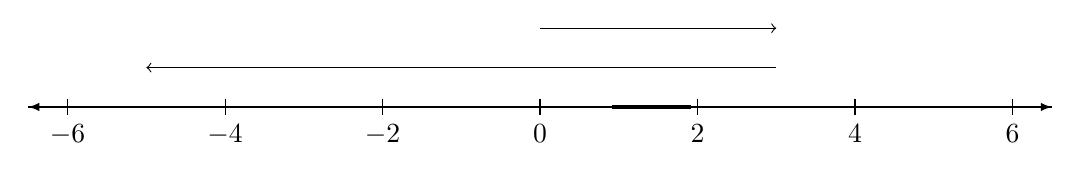
\begin{tikzpicture}
    \draw[latex-] (-6.5,0) -- (6.5,0) ;
    \draw[-latex] (-6.5,0) -- (6.5,0) ;
    \foreach \x in  {-6,-4,-2,0,2,4,6}
    \draw[shift={(\x,0)},color=black] (0pt,3pt) -- (0pt,-3pt);
    \foreach \x in {-6,-4,-2,0,2,4,6}
    \draw[shift={(\x,0)},color=black] (0pt,0pt) -- (0pt,-3pt) node[below] 
    {$\x$};
    \draw[->] (0,1.0) -- (3,1.0);
    \draw[->] (3,0.5) -- (-5,0.5);
    \draw[very thick    ] (0.92,0) -- (1.92,0);
    \end{tikzpicture}"""%
\end{document}